% -*- root: Dissertation.tex -*-
\documentclass[Dissertation.tex]{subfiles} 
\begin{document}

\chapter{Positronium Hydride and Short-Range Terms}
\label{chp:PsHBound}

\iftoggle{UNT}{As}{\lettrine{\textcolor{startcolor}{A}}{s}}
discussed in \cref{sec:PsH}, PsH 
consists of one atom of both Ps and of H.
%We model it the 
%standard way here as an exotic atom, instead of a molecule.
\Cref{fig:PsHCoords} shows the PsH coordinate system. There are 6 interparticle 
coordinates, given by $r_1$, $r_2$, $r_3$, $r_{12}$, $r_{13}$, and $r_{23}$. 
The proton is considered infinitely heavy in this treatment.
Armour et al.~\cite{Armour2005} point out that positronium antihydride is an
equivalent system, assuming CPT symmetry. Another related system is e$^+$PsH,
which is stable and can be thought of as e$^+$ orbiting around PsH \cite{Armour2005}.

\begin{figure}
	\centering
	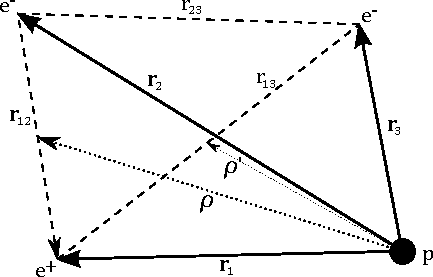
\includegraphics[height=3in]{PsHCoordinates}
	\caption{Positronium hydride coordinate system}
	\label{fig:PsHCoords}
\end{figure}
% If someone gets picky about the fonts here, I could do this instead:
%  http://www.howtotex.com/tips-tricks/inkscape-images-with-latex-fonts/


\section{PsH Wavefunction}
\label{sec:BoundWavefn}

The wavefunction we use for the bound state has a Hylleraas-style
\cite{Yan1999,VanReeth2003} set of terms, given by
\begin{subequations}
\label{eq:BoundWavefn}
\begin{align}
 \Psi^\pm &= \sum_{i=1}^{N(\omega)} c_i \bar{\phi}_i^\pm \label{eq:BoundWavefn_psi} \\
 \bar{\phi}_i^\pm &= (1 \pm P_{23}) \phi_i \label{eq:BoundWavefn_phibar} \\
 \phi_i &= e^{-(\alpha r_1 + \beta r_2 + \gamma r_3)} r_1^{k_i} r_2^{l_i} r_{12}^{m_i} r_3^{n_i} r_{13}^{p_i} r_{23}^{q_i} \label{eq:BoundWavefn_phi} \, ,
\end{align}
\end{subequations}
where the plus sign indicates the spatially symmetric singlet case, and the 
minus sign indicates the spatially antisymmetric triplet case. The 
permutation operator $P_{23}$ is needed, as the two electrons are 
indistinguishable. The $\frac{1}{\sqrt{2}}$ needed to normalize $\Psi^\pm$
(to cancel out the 2 in \cref{eq:RRfinal}) is absorbed into the $c_i$ constant 
in \cref{eq:BoundWavefn_psi}. The constant
$\SphericalHarmY{0}{0}{\theta}{\phi} = \frac{1}{\sqrt{4\pi}}$ is also absorbed
into $c_i$. The Hylleraas-type basis set satisfies the Kato cusp condition
\cite{Kato1957} well \cite{Armour1991}.
% For clarity in some equations, the definition $d_i = \frac{1}{\sqrt{4\pi}} c_i$ is used.

The variable $\omega$ is an integer $\geq 0$ that determines the number of 
terms in the basis set. For a chosen value of $\omega$, the integer powers of 
$r_i$ and $r_{ij}$ are constructed in such a way that \cite{VanReeth2003}
\beq
\label{eq:OmegaDef}
k_i + l_i + m_i + n_i + p_i + q_i \leq \omega,
\eeq
with all $k_i$, $l_i$, $m_i$, $n_i$, $q_i$ and $p_i$ $\geq 0$. 
Using combination with repetition, an explicit formula for $N(\omega)$ is 
given as
\beq
\label{eq:NumberTermsOmega}
N(\omega) = \Binomial{\omega+6}{6} \, ,
\eeq
where the 6 comes from the 6 coordinates of $r_i$ and $r_{ij}$. A plot of
$N(\omega)$ versus $\omega$ is given in \cref{fig:num-omega}.
\begin{figure}
	\centering
	%\scalebox{1}{\includegraphics{NOmega}}
	\includegraphics[width=4in]{num-omega}
	\caption{$N(\omega)$ versus $\omega$}
	\label{fig:num-omega}
\end{figure}


\section{Rayleigh-Ritz Variational Method}
\label{sec:RayleighRitz}
The Rayleigh-Ritz variational method is given as the functional \cite{Bransden2003}
\beq
\label{eq:RayleighRitz}
E[\Psi] = \frac{\Braket{\Psi | H | \Psi}}{\Braket{\Psi | \Psi}}.
\eeq
This provides an upper bound to the ground-state energy, $E_0$. In other words,
\beq
E_0 \leq E[\Psi].
\eeq
\Cref{eq:RayleighRitz} can be rewritten in matrix notation as a generalized eigenvalue problem
\cite{RayleighRitz}
\beq
\label{eq:BoundGenEig}
\textbf{Hc} = E\textbf{Sc},
\eeq
where
\beq
\label{eq:HijSij}
H_{ij} = \left< \bar{\phi}_i \left| H \right| \bar{\phi}_j \right>\!, \, S_{ij} = \left< \bar{\phi}_i \left| \right.\! \bar{\phi}_j \right>, 
\eeq
and \textbf{c} is the vector of coefficients for the wavefunction $\Psi$. The
normalization here is unimportant due to the division in \cref{eq:RayleighRitz}
and the form of \cref{eq:BoundGenEig}.

For PsH, the non-relativistic Hamiltonian is
\beq
\label{eq:BoundHamiltonian}
H = -\frac{1}{2} \Laplacian_{r_1} - \frac{1}{2} \Laplacian_{r_2} - \frac{1}{2} \Laplacian_{r_3} + \frac {1}{r_1}-\frac {1}{r_2}-\frac {1}{r_3}-\frac {1}{r_{12}}-\frac {1}{r_{13}}+\frac {1}{r_{23}}.
\eeq
The Laplacians in \cref{eq:BoundHamiltonian} are complicated when applied to the $\phi_j$ function.  We exploit the short-range nature of $\phi_i$ and $\phi_j$ by using integration by parts, similar to equation (3.21) of Armour and Humberston \cite{Armour1991}.
\beq
\label{eq:BoundGradient}
-\Int{ \phi_i \left(\Laplacian_{r_1} + \Laplacian_{r_2} + \Laplacian_{r_3} \right) \phi_j }{\tau} = \int \sum_{l=1}^3 \grad_{\!\bm{r}_l} \phi_i \bm{\cdot} \grad_{\!\bm{r}_l} \phi_j \, d\tau
\eeq
The differential $d\tau$ represents the 9-dimensional configuration 
space given by $r_1$, $r_2$, and $r_3$ (see \cref{chp:AngularInt}).
This expression is simpler than 
applying the Laplacian operators directly to $\phi_j$, and the summation is 
given by the following expression (a full derivation is given on the research 
Wiki \cite{Wiki}):
\begin{align}
\label{eq:GradGradShort}
\nonumber \sum_{l=1}^3 \grad_{\!\mathbf{r}_l} \phi_i \bm{\cdot} \grad_{\!\mathbf{r}_l} \phi_j = &\phi_i \phi_j \Bigg\{(\alpha^2 + \beta^2 + \gamma^2) - \frac{\alpha}{r_1}(k_i + k_j) - \frac{\beta}{r_2}(l_i + l_j) + \frac{\gamma}{r_3}(n_i + n_j) \\
\nonumber  &+ \frac{k_i k_j}{r_1^2} + \frac{l_i l_j}{r_2^2} + \frac{n_i n_j}{r_3^2} + \frac{2 m_i m_j}{r_{12}^2} + \frac{2 p_i p_j}{r_{13}^2} + \frac{2 q_i q_j}{r_{23}^2} \\
\nonumber  &+ \frac{r_1^2 + r_{12}^2 - r_2^2}{2 r_1^2 r_{12}^2} \left[-\alpha r_1(m_i+m_j) + (k_i m_j + k_j m_i)\right] \\
\nonumber  &+ \frac{r_1^2 + r_{13}^2 - r_3^2}{2 r_1^2 r_{13}^2} \left[-\alpha r_1(p_i+p_j) + (k_i p_j + k_j p_i)\right] \\
\nonumber  &+ \frac{r_{12}^2 + r_{13}^2 - r_{23}^2}{2 r_{12}^2 r_{13}^2} \left[m_i p_j + m_j p_i\right] \\
\nonumber  &+ \frac{r_2^2 + r_{12}^2 - r_1^2}{2 r_2^2 r_{12}^2} \left[-\beta r_2(m_i+m_j) + (m_i l_j + m_j l_i)\right] \\
\nonumber  &+ \frac{r_2^2 + r_{23}^2 - r_3^2}{2 r_2^2 r_{23}^2} \left[-\beta r_2(q_i+q_j) + (l_i q_j + l_j q_i)\right] \\
\nonumber  &+ \frac{r_{12}^2 + r_{23}^2 - r_{13}^2}{2 r_{12}^2 r_{23}^2} \left[m_i q_j + m_j q_i\right] \\
\nonumber  &+ \frac{r_3^2 + r_{13}^2 - r_1^2}{2 r_3^2 r_{13}^2} \left[-\gamma r_3(p_i+p_j) + (n_i p_j + n_j p_i)\right] \\
\nonumber  &+ \frac{r_3^2 + r_{23}^2 - r_2^2}{2 r_3^2 r_{23}^2} \left[-\gamma r_3(q_i+q_j) + (n_i q_j + n_j q_i)\right] \\
		   &+ \frac{r_{13}^2 + r_{23}^2 - r_{12}^2}{2 r_{13}^2 r_{23}^2} \left[p_i q_j + p_j q_i\right] \Bigg\}.
\end{align}
This is similar to the forms given in Refs.~\cite{Armour1991,VanReethThesis}.
The S-wave code also has an alternate formalism using the Laplacian, as given in
Ref.~\cite{Yan1997}.

The full expression for $H_{ij}$ from \cref{eq:HijSij} for real-valued $\phi$
after using \cref{eq:BoundHamiltonian,eq:BoundGradient} is then
\beq
\label{eq:BoundHFull}
\left< \bar{\phi}_i \left| H \right| \bar{\phi}_j \right> = \bigintsss{ \left[ \frac{1}{2}\sum_{l=1}^3 \grad_{\!\mathbf{r}_l} \bar{\phi}_i \boldsymbol{\cdot} \grad_{\!\mathbf{r}_l} \bar{\phi}_j + \left( \frac {1}{r_1}-\frac {1}{r_2}-\frac {1}{r_3}-\frac {1}{r_{12}}-\frac {1}{r_{13}}+\frac {1}{r_{23}} \right) \bar{\phi}_i \bar{\phi}_j \right]}{d\tau}.
\eeq
To reduce the number of integrations needed by half, we use a property of the
permutation operator. Since 
\beq
\left< \phi_i \left| H \right| \phi_j \right> = \left< P_{23} \phi_i \left| H \right| P_{23} \phi_j \right>
\eeq
and
\beq
\left< \phi_i \left| H \right| P_{23} \phi_j \right> = \left< P_{23} \phi_i \left| H \right| \phi_j \right>,
\eeq
\cref{eq:BoundHFull} becomes
\begin{subequations}
\label{eq:RRfinal}
\begin{align}
\nonumber \left< (1 \pm P_{23}) \phi_i \left| H \right| (1 \pm P_{23}) \phi_j \right> =& \left< \phi_i \left| H \right| \phi_j \right> \pm \left< P_{23} \phi_i \left| H \right| \phi_j \right> \\
&\pm \left< \phi_i \left| H \right| P_{23} \phi_j \right> + \left< P_{23} \phi_i \left| H \right| P_{23} \phi_j \right> \\
=& 2 \left[ \left< \phi_i \left| H \right| \phi_j \right> \pm \left< P_{23} \phi_i \left| H \right| \phi_j \right> \right] \\
=& 2 \left[ \left< \phi_i \left| H \right| \phi_j \right> \pm \left< \phi_i \left| H \right| P_{23} \phi_j \right> \right].
\end{align}
\end{subequations}




\section{Results}
\label{sec:BoundResults}

The binding energy (also known as the dissociation energy) is given by Ref.~\cite{Page1974} as
\beq
\label{eq:DissociationE}
E_d = -E_1 - \frac{3}{4} \text{ a.u.}
\eeq

The $-\frac{3}{4}$ comes from adding the ground state energies of Ps and H. 
If the PsH system has a lower energy than $-\frac{3}{4}$, the system is bound. 
%Alternatively, if the binding energy is greater than 0, the system is bound.
Using the accurate Bubin and Adamowicz energy in \cref{tab:BoundEnergyOther}, 
this gives that $^1$S PsH is stable against dissociation into Ps and H by
$\SI{0.039 196 765 251}{au}$ or $\SI{1.066 598 271 959}{eV}$. 

\subsection{Bound State: Singlet}
\label{sec:BoundSinglet}

\setlength{\abovecaptionskip}{6pt}   % 0.5cm as an example
\setlength{\belowcaptionskip}{6pt}   % 0.5cm as an example
\begin{table}
\small
\centering
\begin{tabular}{c c c c c c c d{1.12}}
\toprule
$\omega$ & Terms & $\alpha$ & $\beta$ & $\gamma$ & Total Energy (a.u.) & Binding Energy (eV) & \multicolumn{1}{c}{$\Delta E$ (a.u.)} \\ [0.5ex]
\midrule
0 & 1 &     0.60 & 0.60 & 1.00 & $-$0.541 492 378 889 & --- & \multicolumn{1}{c}{---} \\
1 & 7 &     0.60 & 0.60 & 1.00 & $-$0.744 334 244 165 & ---               &  0.202 841 865 276 \\
2 & 28 &    0.60 & 0.60 & 1.00 & $-$0.778 357 106 972 & 0.771 636 156 726 &  0.034 022 862 807 \\
3 & 84 &    0.60 & 0.60 & 1.00 & $-$0.786 807 448 395 & 1.001 581 651 009 &  0.008 450 341 423 \\
4 & 210 &   0.60 & 0.60 & 1.00 & $-$0.788 685 563 109 & 1.052 687 753 648 &  0.001 878 114 714 \\
5 & 462 &   0.60 & 0.60 & 1.00 & $-$0.789 082 645 582 & 1.063 492 917 716 &  0.000 397 082 473 \\
6 & 916 &   0.60 & 0.60 & 1.00 & $-$0.789 169 509 836 & 1.065 856 614 384 &  0.000 086 864 254 \\
7 & 1585 &  0.60 & 0.60 & 1.00 & $-$0.789 189 568 390 & 1.066 402 435 425 &  0.000 020 058 554 \\
8 & 1925 &  0.60 & 0.60 & 1.00 & $-$0.789 194 559 324 & 1.066 538 245 640 &  0.000 004 990 934 \\
9 & 2166 &  0.60 & 0.60 & 1.00 & $-$0.789 195 830 870 & 1.066 572 846 182 &  0.000 001 271 546 \\
10 & 2205 & 0.60 & 0.60 & 1.00 & $-$0.789 196 323 586 & 1.066 586 253 647 &  0.000 000 492 716 \\
11 & 1674 & 0.58 & 0.60 & 1.00 & $-$0.789 196 284 600 & 1.066 585 192 793 & -0.000 000 038 986 \\
\bottomrule
\end{tabular}
\caption{Ground state energy of PsH}
\label{tab:BoundEnergyOld}
\end{table}

The original double precision PsH code was run for a simple choice of the nonlinear parameters $\alpha$, $\beta$ and $\gamma$. During these initial runs, LAPACK returned valid energies through $\omega = 5$. With the $\omega = 6$ runs, it had trouble using the full 924 terms, with \texttt{dsygv} giving an error. Using Todd's algorithm (\cref{sec:ToddBound}), this code returned a usable 916 terms for $\omega = 6$, as given in \cref{tab:BoundEnergyOld}. The original code worked well through $\omega = 10$, but going from $\omega = 9$ to $\omega = 10$ only added an additional 39 terms. The run for $\omega = 11$ was obviously a problem, since it gave less terms than $\omega = 10$ and a higher energy, even when changing the $\alpha$ parameter slightly.

\setlength{\abovecaptionskip}{6pt}   % 0.5cm as an example
\setlength{\belowcaptionskip}{6pt}   % 0.5cm as an example
\begin{table}
\small
\centering
\centerline{
\begin{tabular}{c c c c c c c c}
\toprule
$\omega$ & Terms & $\alpha$ & $\beta$ & $\gamma$ & Total Energy (a.u.) & Binding Energy (eV) & $\Delta E$ (a.u.) \\ [0.5ex]
\midrule
0 & 1    & 0.586 & 0.580 & 1.093 & -0.558 977 058 051 & --- & --- \\
1 & 7    & 0.586 & 0.580 & 1.093 & -0.744 698 936 920 & ---               & 0.185 721 878 869 \\
2 & 28   & 0.586 & 0.580 & 1.093 & -0.778 246 602 473 & 0.768 629 176 247 & 0.033 547 665 553 \\
3 & 84   & 0.586 & 0.580 & 1.093 & -0.786 743 703 126 & 0.999 847 053 924 & 0.008 497 100 653 \\
4 & 210  & 0.586 & 0.580 & 1.093 & -0.788 672 801 036 & 1.052 340 479 962 & 0.001 929 097 910 \\
5 & 462  & 0.586 & 0.580 & 1.093 & -0.789 082 645 582 & 1.063 460 197 197 & 0.000 409 844 546 \\
6 & 924  & 0.586 & 0.580 & 1.093 & -0.789 169 509 836 & 1.065 861 354 038 & 0.000 086 864 254 \\
7 & 1716 & 0.586 & 0.580 & 1.093 & -0.789 189 730 694 & 1.066 406 851 931 & 0.000 020 220 858 \\
\bottomrule
\end{tabular}
}
\caption{Ground state energy of $^1$S PsH with full set of terms and original ordering}
\label{tab:BoundEnergy1}
\end{table}

The next and current version of the code uses quadruple precision and is able 
to do full runs through $\omega = 8$ without omitting terms (not shown in 
\cref{tab:BoundEnergy1}). Linear dependence is also decreased when the 
nonlinear parameters are different (\cref{sec:BoundOptimization} for 
parameter optimization). The Ps-H scattering problem (\cref{chp:SWave}) is 
more difficult, so a run with $\omega = 7$ is all that is needed.
\Cref{tab:BoundEnergy1} shows the PsH energies through $\omega = 7$ for the full 
set of terms described by \cref{eq:OmegaDef}.

%\setlength{\abovecaptionskip}{6pt}   % 0.5cm as an example
%\setlength{\belowcaptionskip}{6pt}   % 0.5cm as an example
%\begin{table}
%\small
%\centering
%\centerline{
%\begin{tabular}{c c c c c c c c}
%\toprule
%$\omega$ & Terms & $\alpha$ & $\beta$ & $\gamma$ & Total Energy (a.u.) & Binding Energy (eV) & $\Delta E$ (au) \\ [0.5ex]
%\midrule
%0 & 1    & 0.586 & 0.580 & 1.093 & -0.667 061 651 939 & --- & --- \\
%1 & 5    & 0.586 & 0.580 & 1.093 & -0.744 026 116 052 & ---               & 0.076 964 464 113 \\
%2 & 25   & 0.586 & 0.580 & 1.093 & -0.782 354 938 988 & 0.880 422 703 095 & 0.038 328 822 936 \\
%3 & 77   & 0.586 & 0.580 & 1.093 & -0.787 040 587 400 & 1.007 925 686 241 & 0.004 685 648 412 \\
%4 & 199  & 0.586 & 0.580 & 1.093 & -0.788 799 610 636 & 1.055 791 144 810 & 0.001 759 023 236 \\
%5 & 436  & 0.586 & 0.580 & 1.093 & -0.789 131 695 127 & 1.064 827 623 779 & 0.000 332 084 491 \\
%6 & 856  & 0.586 & 0.580 & 1.093 & -0.789 188 377 502 & 1.066 370 029 703 & 0.000 056 682 375 \\
%7 & 1505 & 0.586 & 0.580 & 1.093 & -0.789 189 725 291 & 1.066 406 704 904 & 0.000 001 347 789 \\
%\bottomrule
%\end{tabular}
%}
%\caption{Ground state energy of $^1$S PsH with Todd set of terms}
%\label{tab:BoundEnergyTodd1}
%\end{table}

\setlength{\abovecaptionskip}{6pt}   % 0.5cm as an example
\setlength{\belowcaptionskip}{6pt}   % 0.5cm as an example
\begin{table}
\small
\centering
\centerline{
\begin{tabular}{c c c c c c c c}
\toprule
$\omega$ & Terms & $\alpha$ & $\beta$ & $\gamma$ & Total Energy (a.u.) & Binding Energy (eV) & $\Delta E$ (a.u.) \\ [0.5ex]
\midrule
0 & 1    & 0.586 & 0.580 & 1.093 & -0.558 977 058 051 & --- & --- \\
1 & 5    & 0.586 & 0.580 & 1.093 & -0.718 445 865 883 & ---               & 0.159 468 807 832 \\
2 & 25   & 0.586 & 0.580 & 1.093 & -0.776 355 701 568 & 0.717 175 143 631 & 0.057 909 835 685 \\
3 & 77   & 0.586 & 0.580 & 1.093 & -0.786 645 720 870 & 0.997 180 821 018 & 0.010 290 019 302 \\
4 & 199  & 0.586 & 0.580 & 1.093 & -0.788 665 304 510 & 1.052 136 489 091 & 0.002 019 583 640 \\
5 & 436  & 0.586 & 0.580 & 1.093 & -0.789 080 739 334 & 1.063 441 046 057 & 0.000 415 434 824 \\
6 & 856  & 0.586 & 0.580 & 1.093 & -0.789 169 644 174 & 1.065 860 269 913 & 0.000 088 904 841 \\
7 & 1505 & 0.586 & 0.580 & 1.093 & -0.789 189 725 050 & 1.066 406 698 333 & 0.000 020 080 875 \\
\bottomrule
\end{tabular}
}
\caption{Ground state energy of $^1$S PsH with Todd set of terms and original ordering}
\label{tab:BoundEnergyTodd1}
\end{table}

As described later in \cref{sec:CompPhase}, we cannot use the full 1716 terms 
for the Ps-H scattering problem. \Cref{tab:BoundEnergyTodd1} gives the ground 
state energies using the restricted set of terms using Todd's method with the 
original ordering. The cutoffs in $\omega$ are easily seen using the
ViewOmegaCutoffs.py script (\cref{chp:Programs}).
%\url{http://cas-bs5cph1.phys.unt.edu/wiki/index.php/ViewOmegaCutoffs.py}

%{
	%\iftoggle{UNT}{\singlespacing}
%
	%\begin{center}
	%\setlength{\aboverulesep}{0pt}
	%\setlength{\belowrulesep}{0pt}
	%\setlength{\extrarowheight}{.75ex}
	%\footnotesize
	%\rowcolors{2}{gray!15}{white}
	%\begin{longtable}{l l c l l}
	%\rowcolors{2}{gray!15}{white}
	%\label{tab:BoundEnergyOther} \\
	%\toprule
	%\rowcolor{gray!25} \multicolumn{1}{c}{} & \multicolumn{1}{c}{} & \multicolumn{1}{c}{} & \multicolumn{1}{c}{Total} & \multicolumn{1}{c}{Binding} \\
	%\rowcolor{gray!25} \multicolumn{1}{c}{Group} & \multicolumn{1}{c}{Method} & \multicolumn{1}{c}{Terms} & \multicolumn{1}{c}{Energy (au)} & \multicolumn{1}{c}{Energy (eV)} \\
	%\midrule
	%\endfirsthead
%
	%\rowcolor{white}\multicolumn{5}{r}{{  }} \\
	%\toprule
	%\rowcolor{gray!25} \multicolumn{1}{c}{} & \multicolumn{1}{c}{} & \multicolumn{1}{c}{} & \multicolumn{1}{c}{Dissociation} & \multicolumn{1}{c}{Binding} \\
	%\rowcolor{gray!25} \multicolumn{1}{c}{Group} & \multicolumn{1}{c}{Method} & \multicolumn{1}{c}{Terms} & \multicolumn{1}{c}{Energy (au)} & \multicolumn{1}{c}{Energy (eV)} \\
	%\midrule
	%\endhead
%
	%\hline \multicolumn{5}{r}{{Continued on next page}} \\ \hline
	%\rowcolor{white} \caption[Positronium hydride energy values]{Positronium hydride energy values. Starred values are the reported values. Unstarred values are obtained by using the conversion factor given in \cref{sec:Units}. Results marked by $^a$ take into account the finite mass correction.} \\
	%\endfoot
%
	%\caption[Positronium hydride energy values]{Continued from previous page. Positronium hydride energy values. Starred values are the reported values. Unstarred values are obtained by using the conversion factor given in \cref{sec:Units}. Results marked by $^a$ take into account the finite mass correction.}
	%\endlastfoot
	%\rowcolors{2}{gray!15}{white}
	%Current work & Variational Hylleraas $(\omega = 7)$ & 1505 & -0.789 189 725 & 1.066 406 705 \\
	%Frolov (2010) \cite{Frolov2010} & Semi-exponential & 84 & -0.788 516 419$^\star$ & 1.048 085 11 \\
	%Bubin (2006) \cite{Bubin2006} & ECGs variational & 5000 & -0.789 196 765 251$^\star$ & 1.066 598 271 959 \\
	%Bubin (2006) \cite{Bubin2006} & ECGs variational$^a$ & 5000 & -0.788 870 710 444$^\star$ & 1.057 725 869 06 \\
	%Mitroy (2006) \cite{Mitroy2006} & ECGs with SVM & 1800 & -0.789 196 740$^\star$ & 1.066 597 58 \\
	%Chiesa (2004) \cite{Chiesa2004} & Quantum Monte Carlo & --- & -0.784 620$^\star$ & 0.942 058 \\
	%Bubin (2004) \cite{Bubin2004} & ECGs$^a$ & 3200 & -0.788 870 706 6$^\star$ & 1.057 725 764 \\
	%Van Reeth (2003) \cite{VanReeth2003} & Variational Hylleraas $(\omega = 6)$ & 721 & -0.789 156 & 1.065 5$^\star$ \\
	%Bressanini (2003) \cite{Bressanini2003} & Variational Monte Carlo & 1 & -0.786 073$^\star$ & 0.981 596 \\
	%Saito (2003) \cite{Saito2003a} & CI & 13230 & -0.786 793$^\star$ & 1.001 19 \\
	%Bromley (2001) \cite{Bromley2001} & CI & 95324 & -0.786 776 1$^\star$ & 1.000 729 \\
	%Saito (2000) \cite{Saito2000} & Hylleraas & 396 & -0.788 951$^\star$ & 1.059 91 \\
	%Bromley (2000) \cite{Bromley2000} & CI & --- & -0.784 301 8$^\star$ & 0.933 399 5 \\
	%Yan (1999) \cite{Yan1999} & Variational Hylleraas $(\omega = 12)$ & 5741 & -0.789 196 705 1$^\star$ & 1.066 596 635 \\
	%Yan (1999) \cite{Yan1999} & Variational Hylleraas $(\omega \rightarrow \infty)$ & --- & -0.789 196 714 7$^\star$ & 1.066 596 896 \\
	%Yan (1999) \cite{Yan1999a} & Variational Hylleraas$^a$ & 4705 & -0.788 853 107$^\star$ & 1.057 246 85 \\
	%Ryzhikh (1999) \cite{Ryzhikh1999} & ECGs & 750 & -0.789 196 0$^\star$ & 1.066 577 \\
	%Adhikari (1999) \cite{Adhikari1999} & Five-state CC & --- & -0.788 6 & 1.05$^\star$ \\
	%Mella (1999) \cite{Mella1999} & DMC & --- & -0.789 15$^\star$ & 1.065 3 \\
	%Ryzhikh (1998) \cite{Ryzhikh1998} & ECGs with SVM & 500 & -0.789 194 4$^\star$ & 1.066 534 \\
	%Strasburger (1998) \cite{Strasburger1998} & ECGs & 332 & -0.789 185$^\star$ & 1.066 278 \\
	%Bressanini (1998) \cite{Bressanini1998} & DMC & --- & -0.789 175$^\star$ & 1.066 01 \\
	%Jiang (1998) \cite{Jiang1998} & DMC & --- & -0.789 18$^\star$ & 1.066 1 \\
	%Jiang (1998) \cite{Jiang1998} & Variational Monte Carlo & 1 & -0.777 4$^\star$ & 0.745 6 \\
	%Le Sech (1998) \cite{LeSech1998} & Variational Monte Carlo & 1 & -0.772 3$^\star$ & 0.606 8 \\
	%Usukura (1998) \cite{Usukura1998} & ECGs with SVM & 1600 & -0.789 196 553 6$^\star$ & 1.066 592 513 \\
	%Frolov (1997) \cite{Frolov1997a} & James-Coolidge variational & 924 & -0.789 136 9$^\star$ & 1.064 969 \\
	%Frolov (1997) \cite{Frolov1997a} & James-Coolidge variational & --- & -0.789 181 8$^\star$ & 1.066 191 \\
	%Frolov (1997) \cite{Frolov1997c} & Kolesnikov-Tarasov variational & --- & -0.789 179 4$^\star$ & 1.066 126 \\
	%Frolov (1997) \cite{Frolov1997c} & Kolesnikov-Tarasov variational$^a$ & --- & -0.788 853 4$^\star$ & 1.057 254 \\
	%Ryzhikh (1997) \cite{Ryzhikh1997} & SVM & 400 & -0.789 183$^\star$ & 1.066 22 \\
	%Yoshida (1996) \cite{Yoshida1996} & DMC & --- & -0.789 1$^\star$ & 1.06$^\star$ \\
	%Saito (1995) \cite{Saito1995a} & Hylleraas & --- & -0.774 71$^\star$ & 0.672 39 \\*
	%Saito (1995) \cite{Saito1995} & Restricted Hartree-Fock & --- & -0.776 & 0.70$^\star$ \\*
	%Strasburger (1995) \cite{Strasburger1995} & CI & --- & -0.763 7$^\star$ & 0.372 8 \\*
	%Strasburger (1995) \cite{Strasburger1995} & SCF & --- & -0.666 9$^\star$ & -2.261 \\*
	%Schrader (1992) \cite{Schrader1992} & Experiment & --- & -0.790 & $1.1 \pm 0.2$ \\*
	%Ho (1986) \cite{Ho1986} & Variational with Hylleraas & 396 & -0.788 945$^\star$ & 1.059 75 \\*
	%Maruyama (1985) \cite{Maruyama1985,Saito2003a} & Hylleraas & --- & -0.788 211$^\star$ & 1.039 77 \\*
	%Ho (1978) \cite{Ho1978} & Variational with Hylleraas & 210 & -0.787 525$^\star$ & 1.021 12$^\star$ \\*
	%Clary (1976) \cite{Clary1976} & Variational & 67 & -0.784 161$^\star$ & 0.929 568 \\*
	%Page (1974) \cite{Page1974} & Variational & 70 & -0.786 79$^\star$ & 1.00 11 \\*
	%Navin (1974) \cite{Navin1974} & Variational & 17 & -0.779 2$^\star$ & 0.794 6 \\*
	%Houston (1973) \cite{Houston1973} & Variational & 56 & -0.774 7$^\star$ & 0.672 5 \\*
	%Lebeda (1969) \cite{Lebeda1969} & Variational & 12 & -0.774 2$^\star$ & 0.658 5 \\*
	%Ludwig (1966) \cite{Ludwig1966} & Configuration interaction & 9 & -0.759 0$^\star$ & 0.244 9 \\*
	%Goldanskii (1964) \cite{Goldanskii1964,Clary1976} & --- & --- & -0.667 7$^\star$ & -2.2395 \\*
	%Neamtan (1962) \cite{Neamtan1962} & Variational exponential & 2 & -0.758 4$^\star$ & 0.228 6 \\*
	%Ore (1951) \cite{Ore1951} & Variational exponential & 2 & -0.752 51$^\star$ & 0.068 301 \\*
	%Walters (2004) \cite{Walters2004} & CC 14Ps14H + H$^-$ & --- & -0.787 9 & 1.03$^\star$\\*
	%Walters (2004) \cite{Walters2004} & CC 9Ps9H + H$^-$ & --- & -0.787 5 & 1.02$^\star$\\*
	%Blackwood (2002) \cite{Blackwood2002} & CC 14Ps14H & --- & -0.786 5  & 0.994$^\star$ \\*
	%Blackwood (2002) \cite{Blackwood2002} & CC 9Ps9H & --- & -0.785 4 & 0.963$^\star$ \\*
	%Blackwood (2002) \cite{Blackwood2002b} & CC 22Ps1H + H$^-$ & --- & -0.781 2 & 0.850$^\star$ \\*
	%Campbell (1998) \cite{Campbell1998} & CC 22Ps1H & --- & -0.773 3 & 0.634$^\star$ \\*
	%\bottomrule
	%\end{longtable}
	%\end{center}
	%%\end{landscape}
%
%}


{
	\iftoggle{UNT}{\singlespacing}

	\begin{center}
	\setlength{\aboverulesep}{0pt}
	\setlength{\belowrulesep}{0pt}
	\setlength{\extrarowheight}{.75ex}
	\footnotesize
	\rowcolors{2}{gray!15}{white}
	\begin{longtable}{l c l l}
	\rowcolors{2}{gray!15}{white}
	\label{tab:BoundEnergyOther} \\
	\toprule
	\rowcolor{gray!25} \multicolumn{1}{c}{} & \multicolumn{1}{c}{} & \multicolumn{1}{c}{Total} & \multicolumn{1}{c}{Binding} \\
	\rowcolor{gray!25} \multicolumn{1}{c}{Group / Method} & \multicolumn{1}{c}{Terms} & \multicolumn{1}{c}{Energy (au)} & \multicolumn{1}{c}{Energy (eV)} \\
	\midrule
	\endfirsthead

	\rowcolor{white}\multicolumn{4}{r}{{  }} \\
	\toprule
	\rowcolor{gray!25} \multicolumn{1}{c}{} & \multicolumn{1}{c}{} & \multicolumn{1}{c}{Dissociation} & \multicolumn{1}{c}{Binding} \\
	\rowcolor{gray!25} \multicolumn{1}{c}{Group / Method} & \multicolumn{1}{c}{Terms} & \multicolumn{1}{c}{Energy (au)} & \multicolumn{1}{c}{Energy (eV)} \\
	\midrule
	\endhead

	\hline \multicolumn{4}{r}{{Continued on next page}} \\ \hline
	\rowcolor{white} \caption[Positronium hydride energy values]{Positronium hydride energy values. Starred values are the reported values. Unstarred values are obtained by using the conversion factor given in \cref{sec:Units}. Results marked by $^a$ take into account the finite mass correction.} \\
	\endfoot

	\caption[Positronium hydride energy values]{Continued from previous page. Positronium hydride energy values. Starred values are the reported values. Unstarred values are obtained by using the conversion factor given in \cref{sec:Units}. Results marked by $^a$ take into account the finite mass correction.}
	\endlastfoot
	\rowcolors{2}{gray!15}{white}
	Current work / Variational Hylleraas $(\omega = 7)$ & 1505 & -0.789 189 725 & 1.066 406 705 \\
	Frolov (2010) \cite{Frolov2010} / Semi-exponential & 84 & -0.788 516 419$^\star$ & 1.048 085 11 \\
	Bubin (2006) \cite{Bubin2006} / ECGs variational & 5000 & -0.789 196 765 251$^\star$ & 1.066 598 271 959 \\
	Bubin (2006) \cite{Bubin2006} / ECGs variational$^a$ & 5000 & -0.788 870 710 444$^\star$ & 1.057 725 869 06 \\
	Mitroy (2006) \cite{Mitroy2006} / ECGs with SVM & 1800 & -0.789 196 740$^\star$ & 1.066 597 58 \\
	Chiesa (2004) \cite{Chiesa2004} / Quantum Monte Carlo & --- & -0.784 620$^\star$ & 0.942 058 \\
	Bubin (2004) \cite{Bubin2004} / ECGs$^a$ & 3200 & -0.788 870 706 6$^\star$ & 1.057 725 764 \\
	Van Reeth (2003) \cite{VanReeth2003} / Variational Hylleraas $(\omega = 6)$ & 721 & -0.789 156 & 1.065 5$^\star$ \\
	Bressanini (2003) \cite{Bressanini2003} / Variational Monte Carlo & 1 & -0.786 073$^\star$ & 0.981 596 \\
	Saito (2003) \cite{Saito2003a} / CI & 13230 & -0.786 793$^\star$ & 1.001 19 \\
	Bromley (2001) \cite{Bromley2001} / CI & 95324 & -0.786 776 1$^\star$ & 1.000 729 \\
	Saito (2000) \cite{Saito2000} / Hylleraas & 396 & -0.788 951$^\star$ & 1.059 91 \\
	Bromley (2000) \cite{Bromley2000} / CI & --- & -0.784 301 8$^\star$ & 0.933 399 5 \\
	Yan (1999) \cite{Yan1999} / Variational Hylleraas $(\omega = 12)$ & 5741 & -0.789 196 705 1$^\star$ & 1.066 596 635 \\
	Yan (1999) \cite{Yan1999} / Variational Hylleraas $(\omega \rightarrow \infty)$ & --- & -0.789 196 714 7$^\star$ & 1.066 596 896 \\
	Yan (1999) \cite{Yan1999a} / Variational Hylleraas$^a$ & 4705 & -0.788 853 107$^\star$ & 1.057 246 85 \\
	Ryzhikh (1999) \cite{Ryzhikh1999} / ECGs & 750 & -0.789 196 0$^\star$ & 1.066 577 \\
	Adhikari (1999) \cite{Adhikari1999} / Five-state CC & --- & -0.788 6 & 1.05$^\star$ \\
	Mella (1999) \cite{Mella1999} / DMC & --- & -0.789 15$^\star$ & 1.065 3 \\
	Ryzhikh (1998) \cite{Ryzhikh1998} / ECGs with SVM & 500 & -0.789 194 4$^\star$ & 1.066 534 \\
	Strasburger (1998) \cite{Strasburger1998} / ECGs & 332 & -0.789 185$^\star$ & 1.066 278 \\
	Bressanini (1998) \cite{Bressanini1998} / DMC & --- & -0.789 175$^\star$ & 1.066 01 \\
	Jiang (1998) \cite{Jiang1998} / DMC & --- & -0.789 18$^\star$ & 1.066 1 \\
	Jiang (1998) \cite{Jiang1998} / Variational Monte Carlo & 1 & -0.777 4$^\star$ & 0.745 6 \\
	Le Sech (1998) \cite{LeSech1998} / Variational Monte Carlo & 1 & -0.772 3$^\star$ & 0.606 8 \\
	Usukura (1998) \cite{Usukura1998} / ECGs with SVM & 1600 & -0.789 196 553 6$^\star$ & 1.066 592 513 \\
	Frolov (1997) \cite{Frolov1997a} / James-Coolidge variational & 924 & -0.789 136 9$^\star$ & 1.064 969 \\
	Frolov (1997) \cite{Frolov1997a} / James-Coolidge variational & --- & -0.789 181 8$^\star$ & 1.066 191 \\
	Frolov (1997) \cite{Frolov1997c} / Kolesnikov-Tarasov variational & --- & -0.789 179 4$^\star$ & 1.066 126 \\
	Frolov (1997) \cite{Frolov1997c} / Kolesnikov-Tarasov variational$^a$ & --- & -0.788 853 4$^\star$ & 1.057 254 \\
	Ryzhikh (1997) \cite{Ryzhikh1997} / SVM & 400 & -0.789 183$^\star$ & 1.066 22 \\
	Yoshida (1996) \cite{Yoshida1996} / DMC & --- & -0.789 1$^\star$ & 1.06$^\star$ \\
	Saito (1995) \cite{Saito1995a} / Hylleraas & --- & -0.774 71$^\star$ & 0.672 39 \\*
	Saito (1995) \cite{Saito1995} / Restricted Hartree-Fock & --- & -0.776 & 0.70$^\star$ \\*
	Strasburger (1995) \cite{Strasburger1995} / CI & --- & -0.763 7$^\star$ & 0.372 8 \\*
	Strasburger (1995) \cite{Strasburger1995} / SCF & --- & -0.666 9$^\star$ & -2.261 \\*
	Schrader (1992) \cite{Schrader1992} / Experiment & --- & -0.790 & $1.1 \pm 0.2$ \\*
	Ho (1986) \cite{Ho1986} / Variational with Hylleraas & 396 & -0.788 945$^\star$ & 1.059 75 \\*
	Maruyama (1985) \cite{Maruyama1985,Saito2003a} / Hylleraas & --- & -0.788 211$^\star$ & 1.039 77 \\*
	Ho (1978) \cite{Ho1978} / Variational with Hylleraas & 210 & -0.787 525$^\star$ & 1.021 12$^\star$ \\*
	Clary (1976) \cite{Clary1976} / Variational & 67 & -0.784 161$^\star$ & 0.929 568 \\*
	Page (1974) \cite{Page1974} / Variational & 70 & -0.786 79$^\star$ & 1.00 11 \\*
	Navin (1974) \cite{Navin1974} / Variational & 17 & -0.779 2$^\star$ & 0.794 6 \\*
	Houston (1973) \cite{Houston1973} / Variational & 56 & -0.774 7$^\star$ & 0.672 5 \\*
	Lebeda (1969) \cite{Lebeda1969} / Variational & 12 & -0.774 2$^\star$ & 0.658 5 \\*
	Ludwig (1966) \cite{Ludwig1966} / Configuration interaction & 9 & -0.759 0$^\star$ & 0.244 9 \\*
	Goldanskii (1964) \cite{Goldanskii1964,Clary1976} / --- & --- & -0.667 7$^\star$ & -2.2395 \\*
	Neamtan (1962) \cite{Neamtan1962} / Variational exponential & 2 & -0.758 4$^\star$ & 0.228 6 \\*
	Ore (1951) \cite{Ore1951} / Variational exponential & 2 & -0.752 51$^\star$ & 0.068 301 \\*
	Walters (2004) \cite{Walters2004} / CC 14Ps14H + H$^-$ & --- & -0.787 9 & 1.03$^\star$\\*
	Walters (2004) \cite{Walters2004} / CC 9Ps9H + H$^-$ & --- & -0.787 5 & 1.02$^\star$\\*
	Blackwood (2002) \cite{Blackwood2002} / CC 14Ps14H & --- & -0.786 5  & 0.994$^\star$ \\*
	Blackwood (2002) \cite{Blackwood2002} / CC 9Ps9H & --- & -0.785 4 & 0.963$^\star$ \\*
	Blackwood (2002) \cite{Blackwood2002b} / CC 22Ps1H + H$^-$ & --- & -0.781 2 & 0.850$^\star$ \\*
	Campbell (1998) \cite{Campbell1998} / CC 22Ps1H & --- & -0.773 3 & 0.634$^\star$ \\*
	\bottomrule
	\end{longtable}
	\end{center}
	%\end{landscape}

}

There have been a large number of calculations of the PsH binding energy over 
the years, starting with Ore's prediction in 1951 that PsH could exist
\cite{Ore1951}. As computing power increased, using a Hylleraas-type basis 
set with hundreds or even thousands of terms became possible
\cite{Ho1978,Ho1986,Yan1999,VanReeth2003}. The Hylleraas-type results were 
the most accurate until very accurate ECG results from Mitroy
\cite{Mitroy2006} and Bubin and Adamowicz \cite{Bubin2004,Bubin2006}. The 
ECGs do not satisfy the Kato cusp condition \cite{Kato1957}, but good
optimization of the basis set can give good results \cite{Mitroy2013}.

Another paper by Frolov \cite{Frolov2010} is more of an introduction of a 
modified basis set to this problem, showing how only 84 terms gives a better 
energy than a much larger Hylleraas set. Yan and Ho \cite{Yan1999} use a 
Hylleraas basis set with 5 sectors that each have different nonlinear 
parameters. Frolov's work essentially uses the same basis set but gives each 
term its own set of nonlinear parameters, optimizing all of them 
simultaneously.

The last six entries of this table give the CC results of the Belfast group. 
These are grouped together to show how different states and pseudostates in 
the CC calculations can give better approximations to the binding energy. It 
is particularly clear that adding the H$^-$ channel vastly improves the 
accuracy.

The Hylleraas binding energy from our work in the first line of the table compares
well with the accurate energies of Refs.~\cite{Bubin2006, Mitroy2006, Yan1999},
but it is not as accurate of a calculation. The purpose of doing the PsH 
calculation was not to get the best result but to test how well the short-
range terms for Ps-H scattering represent the short-range interactions. Based 
on \cref{tab:BoundEnergyOther}, the short-range interactions are described 
well. This also gave experience working with the Hylleraas basis set, and 
finding the PsH energy is a simpler problem than Ps-H scattering.

\subsection{Triplet Energy Eigenvalues}
\label{sec:TripletEigenvalues}

Our code does not predict a triplet bound state. Mitroy and Bromley have 
published a paper \cite{Mitroy2007} claiming a stable triplet bound state, 
but our code does not have the appropriate type of wavefunction to see this, 
since it is for a H($2p$) + Ps($2p$) state. They also use a very large 
configuration interaction basis, and this bound state is very shallow. 

Despite not predicting a bound state, we run the energy eigenvalue code for 
the triplet so that we can use this for the short-range terms for the 
scattering programs. The triplet case was more sensitive to the accuracy of 
the matrix elements. Changing the energy eigenvalue code to quadruple 
precision let us use more short-range terms in our calculations.

%With the singlet, 
%we were able to use the full $\omega = 6$ set (924 terms) without the 
%asymptotic expansion before linear dependence became an issue. With the 
%triplet, we were only able to use 450 terms out of an $\omega = 7$ run if the 
%asymptotic expansion was not used. Adding the asymptotic expansion in double 
%precision let us use 1327 terms. Finally, changing the code to quadruple 
%precision lets us use the full set of 1716 terms for an $\omega = 7$ run, as 
%shown in \cref{tab:BoundEnergy3}. 

\setlength{\abovecaptionskip}{6pt}   % 0.5cm as an example
\setlength{\belowcaptionskip}{6pt}   % 0.5cm as an example
\begin{table}
\centering
\begin{tabular}{c c c c c c c}
\toprule
$\omega$ & Terms & $\alpha$ & $\beta$ & $\gamma$ & Total Energy (a.u.) & $\Delta E$ (a.u.) \\ [0.5ex]
\midrule
0 & 1    & 0.323 & 0.334 & 0.975 & -0.500 031 146 247 & --- \\
1 & 7    & 0.323 & 0.334 & 0.975 & -0.623 725 636 031 & 0.123 694 489 784 \\
2 & 28   & 0.323 & 0.334 & 0.975 & -0.679 176 805 541 & 0.055 451 169 510 \\
3 & 84   & 0.323 & 0.334 & 0.975 & -0.710 407 818 871 & 0.031 231 013 330 \\
4 & 210  & 0.323 & 0.334 & 0.975 & -0.727 102 619 903 & 0.016 694 801 032 \\
5 & 462  & 0.323 & 0.334 & 0.975 & -0.735 860 693 040 & 0.008 758 073 137 \\
6 & 924  & 0.323 & 0.334 & 0.975 & -0.740 622 381 908 & 0.004 761 688 868 \\
7 & 1716 & 0.323 & 0.334 & 0.975 & -0.743 386 825 704 & 0.002 764 443 796 \\
\bottomrule
\end{tabular}
\caption{Eigenvalues of $^3$S with full set of terms and original ordering}
\label{tab:BoundEnergy3}
\end{table}

Similar to the singlet, we cannot use the full 1716 
terms for the Ps-H scattering problem. \Cref{tab:BoundEnergyTodd3} gives the 
energy eigenvalues using the restricted set of terms using Todd's method
with original ordering. 

\setlength{\abovecaptionskip}{6pt}   % 0.5cm as an example
\setlength{\belowcaptionskip}{6pt}   % 0.5cm as an example
\begin{table}
\centering
\begin{tabular}{c c c c c c c}
\toprule
$\omega$ & Terms & $\alpha$ & $\beta$ & $\gamma$ & Total Energy (a.u.) & $\Delta E$ (a.u.) \\ [0.5ex]
\midrule
0 & 1    & 0.323 & 0.334 & 0.975 & -0.500 031 146 247 & --- \\
1 & 7    & 0.323 & 0.334 & 0.975 & -0.623 725 636 031 & 0.123 694 489 784 \\
2 & 27   & 0.323 & 0.334 & 0.975 & -0.679 173 632 477 & 0.055 447 996 446 \\
3 & 81   & 0.323 & 0.334 & 0.975 & -0.710 405 860 558 & 0.031 232 228 081 \\
4 & 201  & 0.323 & 0.334 & 0.975 & -0.727 100 988 826 & 0.016 695 128 267 \\
5 & 432  & 0.323 & 0.334 & 0.975 & -0.735 860 470 972 & 0.008 759 482 146 \\
6 & 854  & 0.323 & 0.334 & 0.975 & -0.740 622 201 811 & 0.004 761 730 840 \\
7 & 1633 & 0.323 & 0.334 & 0.975 & -0.743 386 893 723 & 0.002 764 691 911 \\
\bottomrule
\end{tabular}
\caption{Eigenvalues of $^3$S with Todd set of terms and original ordering}
\label{tab:BoundEnergyTodd3}
\end{table}


\section{Stabilization}

Hazi and Taylor \cite{Hazi1970} introduced the concept of stabilization plots 
to PsH bound state calculations.
%This can allow calculations of scattering 
%parameters from a fully bound state calculation.
Specifically, they plotted 
the four lowest eigenvalues with respect to $N$ and looked for avoided 
crossings. A resonance only exists if there is an avoided crossing between 
eigenvalues. The avoided crossing that they found at $\SI{0.428 985}{a.u.}$ (or 
$\SI{5.8366}{eV}$ as shown in \cref{tab:SWaveResonancesOther}) corresponds 
roughly with the first $^1$S resonance. Van Reeth and Humberston \cite{
VanReeth2004} also did an analysis of stabilized eigenvalues but with the 
same type of basis set that we use.

\begin{figure}
	\centering
	\includegraphics[width=4.5in]{swavesinglet-eigen}
	\caption[$^1$S eigenvalues]{$^1$S eigenvalues. The dashed line represents the Ps(n=2) threshold. Dotted lines represent complex Kohn $^1$S resonance positions. The red rectangles are potential avoided crossings.}
	\label{fig:swavesinglet-eigen}
\end{figure}

Plotting the first 10 eigenvalues with respect to $N$ for $^1$S gives
\cref{fig:swavesinglet-eigen}. As noted, the dashed line represents the Ps(n=2) 
inelastic threshold at $\SI{5.102}{eV}$. The dotted lines correspond to the 
first two complex Kohn $^1$S resonance positions given in
\cref{tab:SWaveResonancesOther}. The wavefunction we use is not optimized for this type of 
analysis, but there is evidence of avoided crossing given by the red 
rectangles in \cref{fig:swavesinglet-eigen}. The position of the plateau in 
between these rectangles corresponds relatively well with the first resonance 
position, $^1E_R$, we find in \cref{tab:SWaveResonancesOther} from the full 
scattering calculations in \cref{chp:SWave}. The line for the second 
resonance lines up with the 5th eigenvalue from roughly 700 to 900 terms and 
with the 6th eigenvalue starting at about 1250 terms. %There is not a clear 
%way to get the resonance positions from this if they are not known 
%previously.
The estimates of the two resonances positions is $\SI{3.99}{eV}$ 
and $\SI{5.03}{eV}$.

Van Reeth and Humberston \cite{VanReeth2004} had difficulty doing the same 
type of stabilization with these Hylleraas-type terms. Other wavefunctions or 
stabilization methods may work better for this system. For instance, Yan and 
Ho \cite{Yan2003} vary a scaling factor and plot the eigenvalue energies
with respect to this.

\begin{figure}
	\centering
	\includegraphics[width=4.5in]{swavetriplet-eigen}
	\caption[$^3$S eigenvalues]{$^3$S eigenvalues. The dashed line represents the Ps(n=2) threshold.}
	\label{fig:swavetriplet-eigen}
\end{figure}

\Cref{fig:swavetriplet-eigen} shows the same type of stabilization plot for
$^3$S. It is clear that below the Ps(n=2) threshold, there are no avoided 
crossings, meaning that there are no resonances in the S-wave triplet for 
this energy range. 

\begin{figure}
	\centering
	\includegraphics[width=4.5in]{pwavesinglet-eigen-unpaired}
	\caption[$^1$P eigenvalues for first symmetry only]{$^1$P eigenvalues for first symmetry only. The dashed line represents the Ps(n=2) threshold. Dotted lines represent complex Kohn $^1$P resonance positions.}
	\label{fig:pwavesinglet-eigen-unpaired}
\end{figure}

\begin{figure}
	\centering
	\includegraphics[width=4.5in]{pwavetriplet-eigen-unpaired}
	\caption[$^3$P eigenvalues for first symmetry only]{$^3$P eigenvalues for first symmetry only. The dashed line represents the Ps(n=2) threshold.}
	\label{fig:pwavetriplet-eigen-unpaired}
\end{figure}

\Cref{fig:pwavesinglet-eigen-unpaired,fig:pwavetriplet-eigen-unpaired} show 
the stabilization plots for the P-wave eigenvalues when only the first 
symmetry (see \cref{sec:PWaveFn}) is evaluated. %Similar to $^3$S, there is no 
%evidence of avoided crossings, or resonances, for $^3$P.
In \cref{fig:pwavetriplet-eigen-unpaired}, linear dependence becomes a 
problem at 957 terms, hence why there is an extra eigenvalue below
zero, which is not actually indicative of a bound state.

In \cref{fig:pwavesinglet-eigen-unpaired}, there is evidence of avoided 
crossings for the first resonance marked by the red rectangles. The second 
avoided crossing is barely noticeable. Taking the fifth eigenvalue at 800 
terms gives $\SI{4.44}{eV}$, which is not very much in line with the accurate 
calculations shown in \cref{tab:PWaveResonancesOther}, including the complex 
Kohn. The second resonance is above the Ps(n=2) threshold here, making it 
physically different from the actual resonance.

\begin{figure}
	\centering
	\includegraphics[width=4.5in]{pwavesinglet-eigen-paired}
	\caption[$^1$P eigenvalues for both symmetries]{$^1$P eigenvalues for both symmetries. The dashed line represents the Ps(n=2) threshold. Dotted horizontal lines represent complex Kohn $^1$P resonance positions. The approximate avoided crossings are denoted by rectangles.}
	\label{fig:pwavesinglet-eigen-paired}
\end{figure}

\begin{figure}
	\centering
	\includegraphics[width=4.5in]{pwavetriplet-eigen-paired}
	\caption[$^3$P eigenvalues for both symmetries]{$^3$P eigenvalues for both symmetries. The dashed line represents the Ps(n=2) threshold.}
	\label{fig:pwavetriplet-eigen-paired}
\end{figure}

\Cref{fig:pwavesinglet-eigen-paired,fig:pwavetriplet-eigen-paired} are also 
for the P-wave, but they use both the first and second symmetries paired. So 
each term number given on the x-axis is actually two terms, i.e. $N = 200$ is 
a total of 400 short-range terms, 200 of the first symmetry and 200 of the 
second symmetry. %It is still clear that $^3$P does not have resonances below 
%the inelastic threshold.

In \cref{fig:pwavesinglet-eigen-paired}, the first resonance position lines 
up relatively well with the full scattering calculations. The second 
resonance is a narrow resonance, and there is an avoided crossing enclosed in 
the dashed blue rectangle. The approximate position of the resonances are 
taken as the fifth and sixth eigenvalues at 1000 terms, which are tabulated 
in \cref{tab:Stabilization} and can be compared to the full complex Kohn 
calculation in \cref{tab:PWaveResonancesOther}.

\begin{figure}
	\centering
	\includegraphics[width=4.5in]{dwavesinglet-eigen-unpaired}
	\caption[$^1$D eigenvalues for first symmetry only]{$^1$D eigenvalues for first symmetry only. The dashed line represents the Ps(n=2) threshold. The dotted line represents the complex Kohn $^1$D resonance position.}
	\label{fig:dwavesinglet-eigen-unpaired}
\end{figure}

\begin{figure}
	\centering
	\includegraphics[width=4.5in]{dwavetriplet-eigen-unpaired}
	\caption[$^3$D eigenvalues for first symmetry only]{$^3$D eigenvalues for first symmetry only. The dashed line represents the Ps(n=2) threshold.}
	\label{fig:dwavetriplet-eigen-unpaired}
\end{figure}

\begin{figure}
	\centering
	\includegraphics[width=4.5in]{dwavesinglet-eigen-paired}
	\caption[$^1$D eigenvalues for both symmetries]{$^1$D eigenvalues for both symmetries. The dashed line represents the Ps(n=2) threshold. The dotted line represents the complex Kohn $^1$D resonance position.}
	\label{fig:dwavesinglet-eigen-paired}
\end{figure}

\begin{figure}
	\centering
	\includegraphics[width=4.5in]{dwavetriplet-eigen-paired}
	\caption[$^3$D eigenvalues for both symmetries]{$^3$D eigenvalues for both symmetries. The dashed line represents the Ps(n=2) threshold.}
	\label{fig:dwavetriplet-eigen-paired}
\end{figure}

To complete the discussion for resonances below the inelastic threshold, the
D-wave stabilization plots for the first symmetry only are in
\cref{fig:dwavesinglet-eigen-unpaired,fig:dwavetriplet-eigen-unpaired}. Compared to 
\cref{fig:dwavesinglet-eigen-paired,fig:dwavetriplet-eigen-paired}, the first 
symmetry obviously is not enough to adequately describe the system. There is 
only one resonance before the threshold, and the fifth eigenvalue is taken at 
924 paired terms in \cref{tab:Stabilization}.


\begin{table}
\centering
\begin{tabular}{c c c}
\toprule
Partial wave & $^1E_R$ & $^2E_R$ \\
\midrule
$^1$S & 3.99 & 5.03  \\
$^1$P & 4.28 & 4.99  \\
$^1$D & 4.73 & ---   \\
\bottomrule
\end{tabular}
\caption{Approximate resonance positions found using stabilization method}
\label{tab:Stabilization}
\end{table}

\Cref{tab:Stabilization} gives the resonance positions found using the 
stabilization method. Despite the fact that this stabilization method does 
not give very accurate resonance positions in this work, we can learn some 
things from these. First, we can determine the number of resonances before 
the Ps(n=2) threshold and where to look for them in the full complex Kohn 
calculations. Secondly, the triplet states do not have resonances before this 
threshold for any of these partial waves. Lastly, for $\ell > 0$, both the 
first and second symmetries are needed to accurately describe the system. The 
first symmetry alone cannot adequately describe the P-wave and D-wave.



\biblio
\end{document}
